%% Introduction
\section{Methods}
%An overview of the physical components in the setup is shown in \autoref{fig:SystemOverview}.
\autoref{fig:SystemOverview} shows a head fitted with an ANC headphone using a reference microphone (1), a headphone loudspeaker (2), an error microphone (3) and a DSP (4).
{
	%\centering
	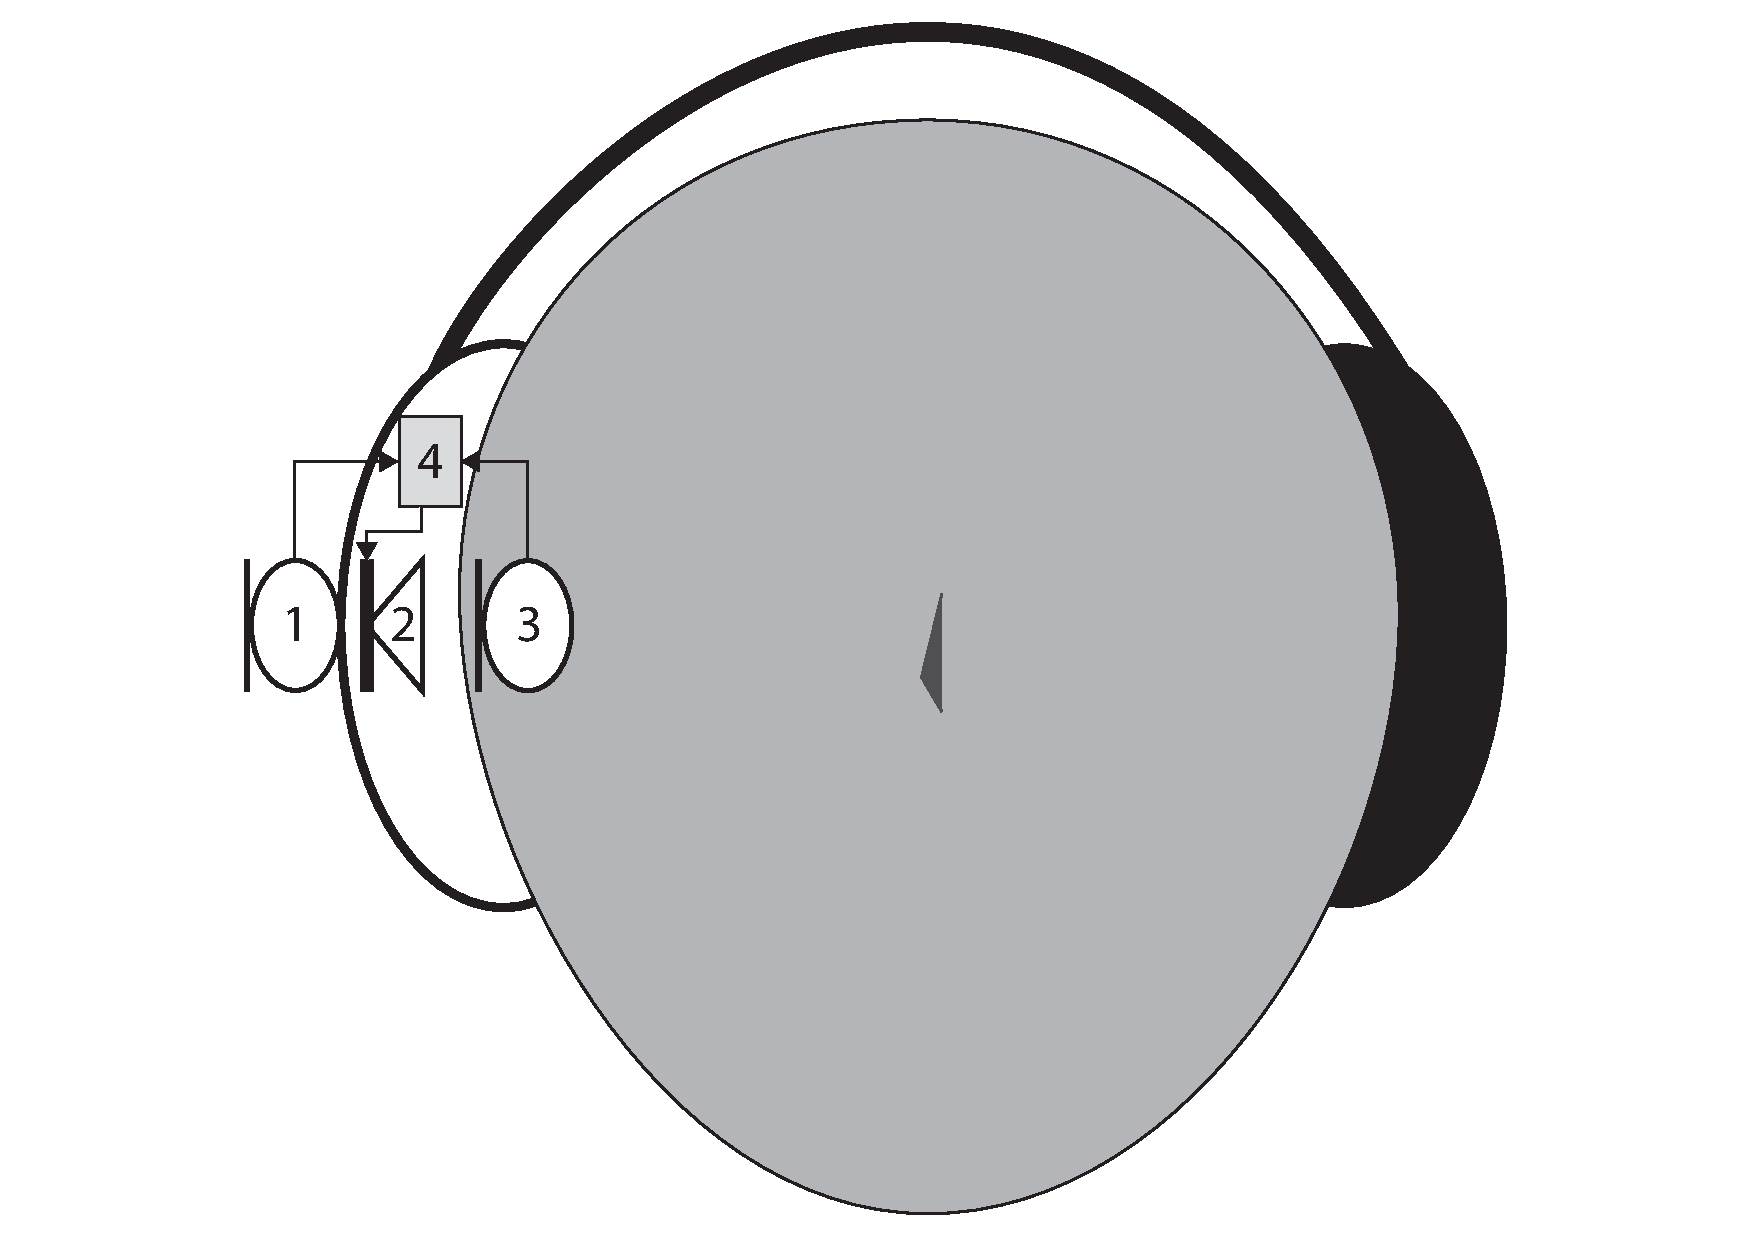
\includegraphics[width=1\columnwidth]{figures/ArticleIllustrations/SystemOverview}
	\captionof{figure}{System Overview.}
	\label{fig:SystemOverview}
}

%\begin{figure}[H]
%	\centering
%	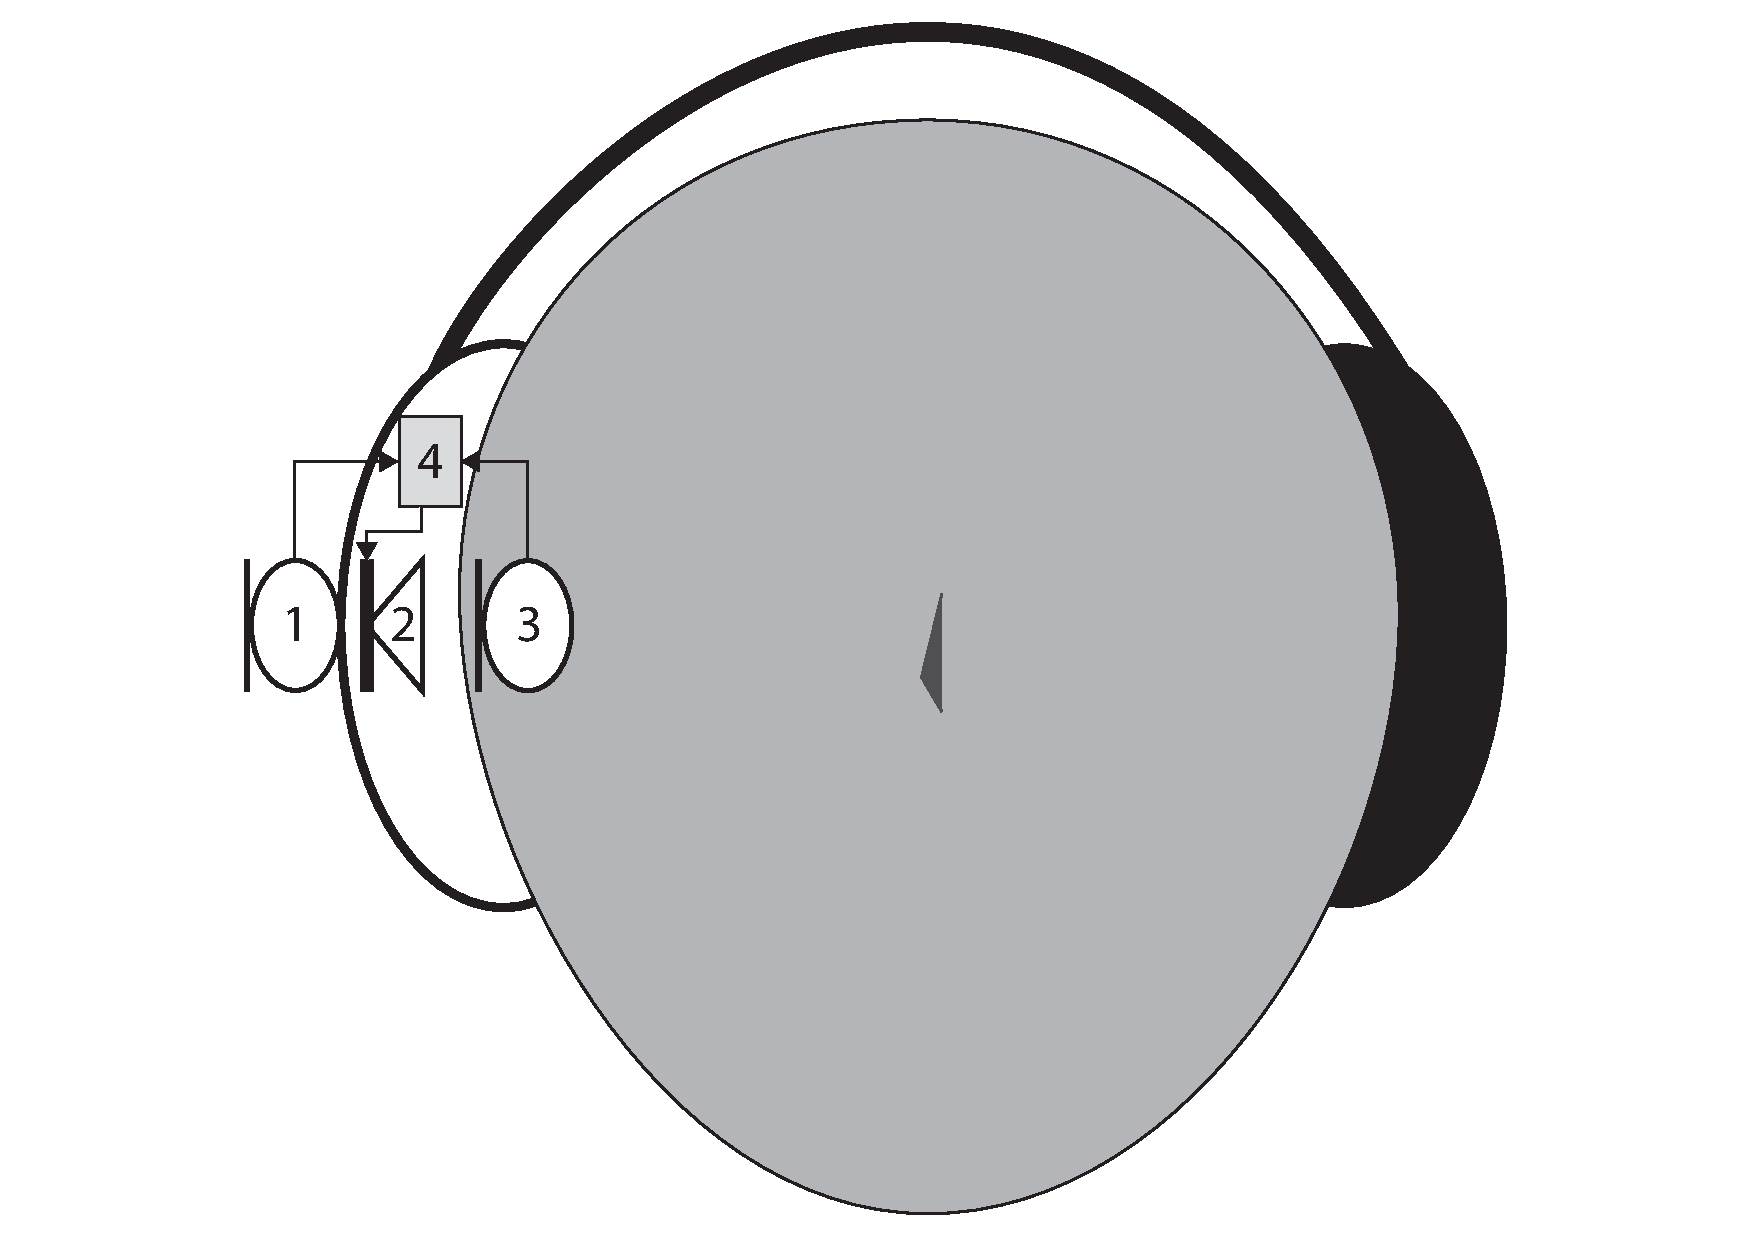
\includegraphics[width=1\columnwidth]{figures/ArticleIllustrations/SystemOverview}
%	\caption{System Overview}
%	\label{fig:SystemOverview}
%\end{figure}



\subsection*{Feedforward ANC using FXLMS}
%The adaptive feedforward ANC system is shown on \autoref{fig:ANCFeedforward}
\autoref{fig:ANCFeedforward} shows an expansion of the DSP-block from \autoref{fig:SystemOverview}. This consists of converters and a control filter which is a FIR filter where the coefficients are adapted by the FXLMS-algorithm. 
{
	%\centering
	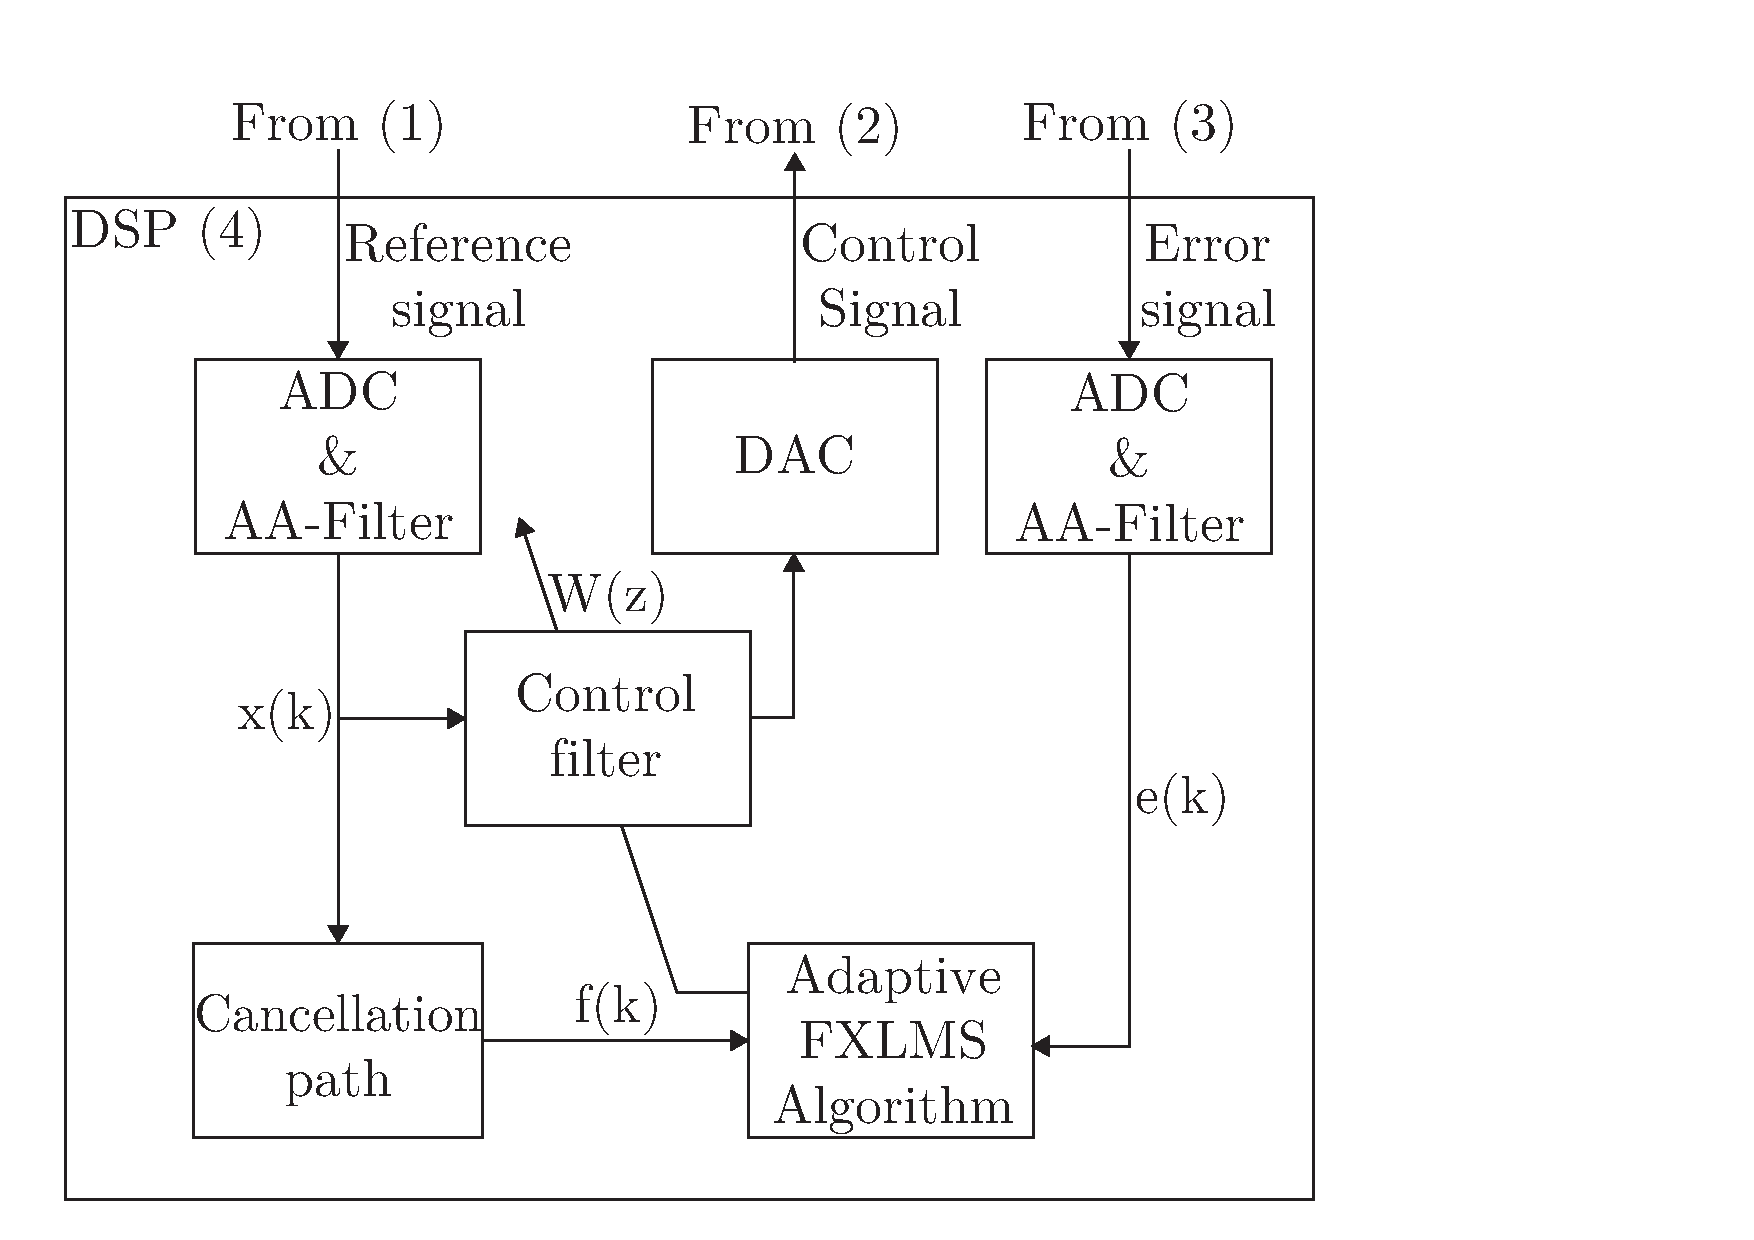
\includegraphics[width=1\columnwidth]{figures/ArticleIllustrations/ANCFeedForward}
	\captionof{figure}{Adaptive feedforward ANC system.}
	\label{fig:ANCFeedforward}
}

%\begin{figure}[H]
%	\centering
%	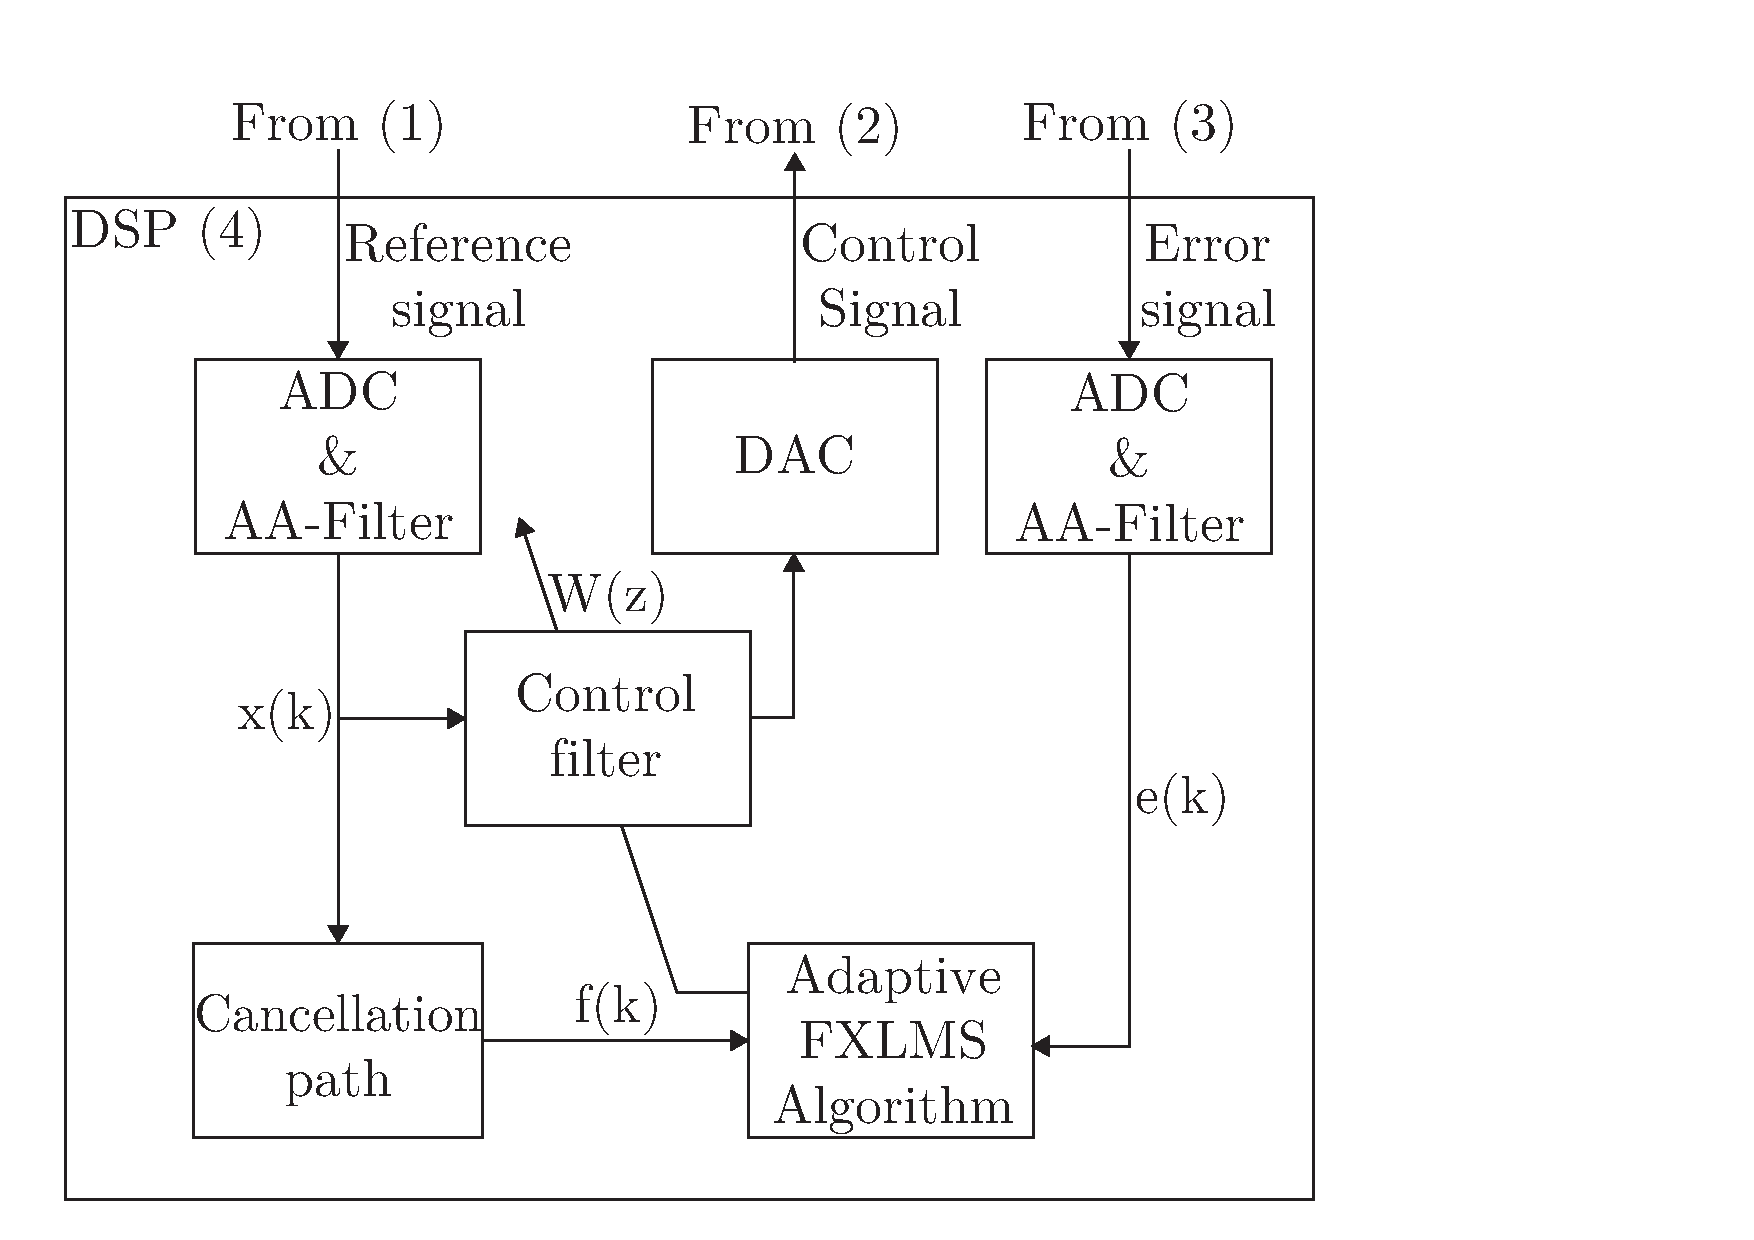
\includegraphics[width=1\columnwidth]{figures/ArticleIllustrations/ANCFeedForward}
%	\caption{Adaptive feedforward ANC system}
%	\label{fig:ANCFeedforward}
%\end{figure}


\textbf{Control Filter} is the filter representing the transfer function from the reference microphone to the headphone loudspeaker. The filter is initialized with the inverse of the first 256 samples from the impulse response of the transfer function found by measurements in \autoref{sec:AngleOfIncidence}.  

\textbf{FXLMS} is the optimization algorithm which updates the control filter coefficients using the FXLMS method shown in \autoref{eq:FXLMS} and derived in \autoref{subsec:fxlms}. 
\begin{equation}\label{eq:FXLMS}
W_j(k+1) = W_j(k) - 2\mu e(k)f(k-j) 
\end{equation}
Where:
\vspace{-8mm} % yeah I know - Sorry Mikkel!
\begin{description}
	\item[\text{$w_j(k)$}] is the weight coefficients of the control filter written as  $w(k)=[w_0(k),w_1(k) \cdots w_{L-1}(k)]^T$
	\item[\text{$\mu$}] is the convergence factor
	\item[\text{$e(k)$}] is the error 
	\item[\text{$f(k)$}] is the reference convolved with the Cancellation Path
\end{description}

\textbf{Cancellation Path} (CP) is the transfer-function from the headphone loudspeaker to the error microphone. In the literature \cite{Hansen} the CP is adaptively adjusted, but it is assumed constant in this setup because the headphone position is fixed.     

\subsection*{Linear Prediction of Speech}
When implementing the system in real-time delays exist due to the anti aliasing and reconstruction filters. The delays of the system exceeds the propagation time of sound from the reference microphone to the headphone loudspeaker resulting in poor performance. Therefore a linear prediction algorithm is proposed to predict future samples in order to decrease the affect of the time delays.


Speech can be split into two main classes, voiced and unvoiced. Voiced sounds are characterized by a strong periodicity in the sound with the fundamental frequency referred to as the pitch frequency (50 - 500 Hz). Unvoiced sounds are characterized as random. Speech is a non stationary and can only be assumed wide sense stationary (WSS) for periods of 20 - 30 ms. Therefore in order to predict future samples the auto correlation function (ACF), which is used in linear prediction, of speech must be estimated in frames. 

%The ACF is estimated using a   

Using the ACF estimator the normal equation shown in \autoref{eq:normal} can be used to derive the linear prediction coefficients (LPCs) which is used for predicting future samples. 
\begin{equation}\label{eq:normal}
R = a\cdot r
\end{equation}
Where:
\vspace{-8mm} % yeah I know - Sorry Mikkel - again!
\begin{description}
	\item[\text{$R$}] is the covariance matrix $C_{xx}$
	\item[\text{$a$}] is the LPCs $a = [a_1 , a_2 \cdots a_M]^T$
	\item[\text{$r$}] is the ACF $r = [R_x[1] , R_x[2] \cdots R_x[M]]^T$
\end{description}
This can be rewritten as shown in \autoref{eq:normal2} yielding the LPCs directly.  
 \begin{equation}\label{eq:normal2}
a = -R^{-1}\cdot r
\end{equation}
However calculating $R^{-1}$ is not possible in a real time application 




